% LaTeX template for MLSP papers. To be used with:
%   * mlspconf.sty - ICASSP/ICIP LaTeX style file adapted for MLSP, and
%   * IEEEbib.bst - IEEE bibliography style file.
% --------------------------------------------------------------------------
\documentclass{article}
\usepackage{amsmath,graphicx,mlspconf}

% Copyright notices.
% ------------------
% Select one of the four copyright notices below. Only required for the camera-ready paper submission.
% 
% * For papers in which all authors are employed by the US government:

% Header
\toappear{EECE5644 Final Project Presentations, Dec.\ 9, 2020, Northeastern University}

% Example definitions.
% --------------------
%\def\x{{\mathbf x}}
%\def\L{{\cal L}}

% Title.
% ------
\title{ANALYSIS OF KALMAN FILTER PERFORMANCE ON LINEAR AND NON-LINEAR VEHICULAR MOTION}
%
% Double-blind peer review.
% -------------------------
% Anonymize your paper for the double-blind peer-review process using the 
% following author and affiliation.
\name{%
    Nathaniel Gordon
    \qquad Eric Grimaldi
    \qquad Siddhant Gupta
}
\address{
    Northeastern University
}

\begin{document}
%\ninept

\maketitle

\begin{abstract}

With the growing prevalence of autonomous vehicles, the need for methods to predict and model the motion of said vehicles is ever increasing. One such method for trajectory estimation is the Kalman filter. In this project, we derive and implement two versions of a Kalman filter that are able to harness RADAR and LIDAR data of a simulated autonomous vehicle to predict the vehicle’s motion with an uncertainty of 4cm. This project demonstrates the effectiveness of the linear and lxtended variations of the Kalman filter, particularly when used in conjunction.

\end{abstract}

\section{Introduction}
\label{sec:intro}

Before proceeding to the applied Kalman filters, the algorithm will be defined in a general sense. The Kalman filter is built around two fundamental phases: the prediction phase, in which a state estimation is produced, and an update phase, during which uncertainty in the state space is propagated for use in the next iteration of the algorithm. The prediction phase can be defined as follows:

$$x' = Fx+u$$

Here, the state space and its projected prediction are denoted $x$ and $x'$ respectively, and $u$ is the control term. $F$ is a representation of the dynamics of the object's motion.

The update phase, in which the future state uncertainty $P'$ is determined, can be represented as a function of the prior uncertainty and measurement noise $Q$:

$$P'=FPF^T+Q$$

Once again, the dynamics matrix $F$ is present. Defining this quantity will be a crucial part of the implementation step.

\section{METHODS}
\label{sec:methods}

\subsection{Linear Kalman Filter Implementation}
\label{ssec:lkfimp}

First, the object dynamics for the autonomous vehicle must be discussed. Two values are pertinent to the prediction of the vehicle's motion: position and velocity. For the linear Kalman filter, linear motion will be assumed:

$$
F = \begin{cases}
p_x'=p_x+v_x\Delta t\\
p_y'=p_y+v_y\Delta t\\
v_x'=v_x\\
v_y'=v_y
\end{cases}
$$

Because there is no aspect of control in this application, we can then represent the prediction equation as:

$$
\begin{pmatrix}
p_x'\\
p_y'\\
v_x'\\
v_y'
\end{pmatrix}=
\begin{pmatrix}
1 && 0 && \Delta t && 0\\
0 && 1 && 0 && \Delta t\\
0 && 0 && 1 && 0\\
0 && 0 && 0 && 1
\end{pmatrix}
\begin{pmatrix}
p_x\\
p_y\\
v_x\\
v_y
\end{pmatrix}
$$

Now, the data may be applied to the algorithm. The data used for this project were borrowed from \cite{gaskey19}. One source of the measurements present in the data is LIDAR. These readings contain a measurement of the vehicle's position in Cartesian space. Let these readings be denoted $z$, the measurement vector:

$$
z = \begin{pmatrix}
p_x\\
p_y
\end{pmatrix}
$$

Because we are unable to directly reason about the vehicle's velocity from the LIDAR input, we will define a mask function $H$ to apply the LIDAR data to only the positional aspects of the state vector:

$$
H = \begin{pmatrix}
1 && 0 && 0 && 0\\
0 && 1 && 0 && 0
\end{pmatrix}
$$

Additionally, the instrument error for the LIDAR readings is 2.25 centimeters.

With these values defined, the update process for the LIDAR readings becomes the following:

$$P'=HPH^T+Q$$

The error, $y$, is the difference between the true reading and the masked projection:

$$y=z-Hx'$$

\begin{figure}[ht]
\begin{minipage}[b]{1.0\linewidth}
  \centering
  \centerline{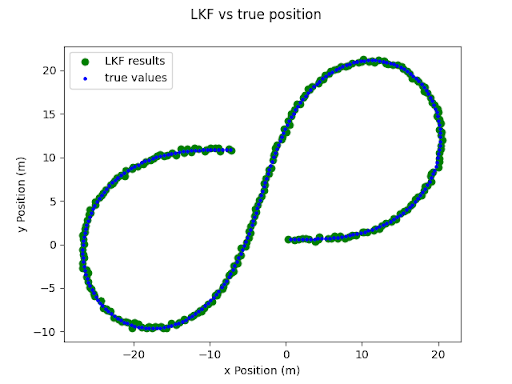
\includegraphics[width=8.5cm]{1.png}}
\end{minipage}
\caption{Positional estimates generated from linear Kalman filter and LIDAR data.}
\end{figure}

Finally, the Kalman gain, $K$, which describes the relative weight placed on the recent measurements (as opposed to older ones), can be derived as thus:

$$K=P'H^TP^I$$



\subsection{Extended Kalman Filter Implementation}
\label{ssec:ekfimp}

The other source of readings in the data is a RADAR system. These readings are given in polar form, and are a description of the vehicle's range $\rho$, perpendicular velocity $\dot{\rho}$, and bearing $\phi$. To convert to Cartesian form, the following transformation is applied:

\begin{figure}[hb]
\begin{minipage}[b]{1.0\linewidth}
  \centering
  \centerline{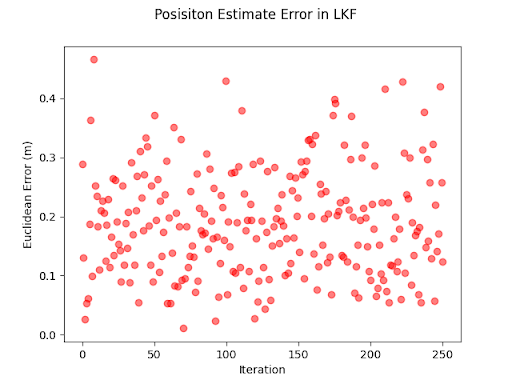
\includegraphics[width=8.5cm]{2.png}}
\end{minipage}
\caption{Error (Euclidean distance) in linear Kalman filter estimation.}
\end{figure}

$$
h(x')=\begin{pmatrix}
\sqrt{p_x'^2+[_y'^2}\\
arctan(p_y'/p_x')\\
\frac{p_x'v_x'+p_y'v_y'}{\sqrt{p_x'^2+p_y'^2}}
\end{pmatrix}
$$

This transformation raises a pertinent issue: it introduces non-linearity into the system. To handle this linearity, the extended Kalman filter methodology is employed.



To adapt the algorithm to account for this non-linearity, the Jacobian of the transformation matrix $h_j$ must be calculated, as derived by \cite{gaskey19}:

$$
h_j=
$$$$\begin{bmatrix}
\frac{p_x}{\sqrt{p_x^2+p_y^2}} && \frac{p_y}{\sqrt{p_x^2+p_y^2}} && 0 && 0\\
-\frac{p_y}{p_x^2+p_y^2} && \frac{p_x}{p_x^2+p_y^2} && 0 && 0\\
\frac{p_y(v_xp_y-v_yp_x)}{(p_x^2+p_y^2)^{3/2}}&& \frac{p_y(v_yp_x-v_xp_y)}{(p_x^2+p_y^2)^{3/2}} && \frac{p_x}{\sqrt{p_x^2+p_y^2}} && \frac{p_y}{\sqrt{p_x^2+p_y^2}}
\end{bmatrix}$$

The rest of the process of constructing the extended Kalman filter is identical to the methods in the previous section, where the linear variant was defined.

\section{RESULTS}
\label{sec:results}

\subsection{Linear Kalman Filter Results}
\label{ssec:lkfresults}

To test the performance of the Kalman filter algorithms, a simplified trial using only LIDAR data was run to isolate the linear Kalman filter algorithm. This meant that while the procedure was unable to produce an estimate of the vehicle's velocity, it could predict its position. The trial contained 250 LIDAR readings of the vehicle traveling in a figure-eight pattern.

\begin{figure}[hb]
\begin{minipage}[b]{1.0\linewidth}
  \centering
  \centerline{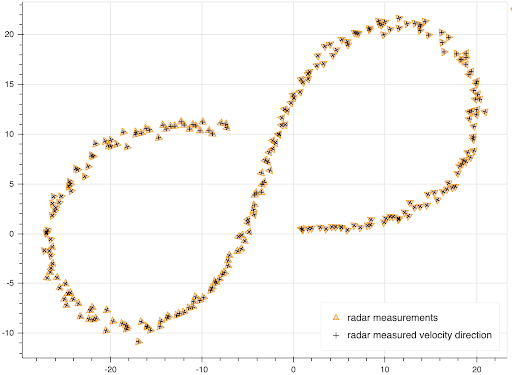
\includegraphics[width=8.5cm]{3.png}}
\end{minipage}
\caption{Compiled LIDAR and RADAR readings from the dataset. The orientation of the triangle markers corresponds to the vehicle's measured bearing.}
\end{figure}

The results of this trial are visible in Figure 1, where the predicted positions are plotted alongside the corresponding true values. Additionally, in Figure 2, the error, found with Euclidean distance from the true value. For this trial, the empirically determined root mean squared error was found to be .21 meters.

While the linear Kalman filter generates accurate predictions of position, it is unable to capture the full state of the vehicle in motion. Thus, subsequent trials were run to determine if using pure RADAR data, or a mix of the two data streams, would improve the prediction quality.

\subsection{Extended Kalman Filter Results}
\label{ssec:ekfresults}

After the linear Kalman filter had been tested independently, a second trial was run, using only the RADAR data from the autonomous vehicle simulation. In this trial, the procedure was able to estimate the complete state vector, capturing both the position and velocity of the vehicle in the prediction. The results of this trial are visible in Figure 4.

Finally, a trial was run where both Kalman filters were run in tandem, analyzing both LIDAR and RADAR data. In estimating the vehicle's motion, the linear Kalman filter serves as the more accurate arbiter of positional data, as it draws from the less noisy LIDAR instrument. However, this model also has the benefit of ascertaining velocity information from the extended Kalman filter. While drawing on the RADAR data is necessary for projecting the vehicle's future state, the graph in Figure 5 demonstrates how the positional data gathered from the extended Kalman filter is much less accurate due to the RADAR's lesser precision. In conjunction, the two filters provide a robust estimation of vehicle movement, drawing from both linear and non-linear data streams.

\begin{figure}[hb]
\begin{minipage}[b]{1.0\linewidth}
  \centering
  \centerline{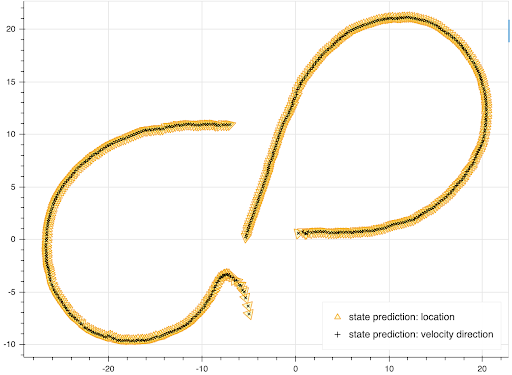
\includegraphics[width=8.5cm]{4.png}}
\end{minipage}
\caption{Predicted vehicle states collected from using only the extended Kalman filter on the RADAR data.}
\end{figure}

\begin{figure}[ht]
\begin{minipage}[b]{1.0\linewidth}
  \centering
  \centerline{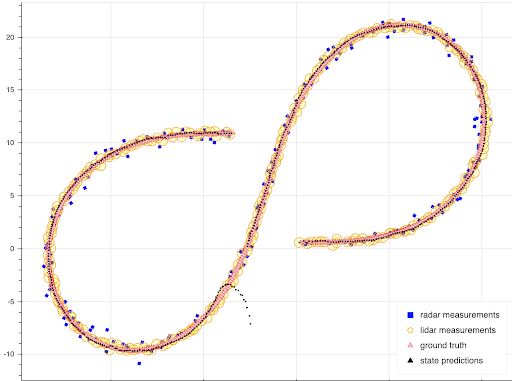
\includegraphics[width=8.5cm]{5.png}}
\end{minipage}
\caption{Overlaid results of drawing predictions from both linear and extended Kalman filters. The state predictions draw on both LIDAR and RADAR data.}
\end{figure}

\section{CONCLUSION}
\label{sec:conclusion}

The outcomes of the three trials indicate that the Kalman filter is a highly flexible tool, and can be used in tandem with other filters to process data from multiple sources. Furthermore, the uncertainty measurement the filter maintains enables it to rely on measurements of different inputs for parts of the state vector, minimizing overall error in the output.

An future extension to this project could entail observing the behavior of the system with changes to the degree of noise in each measuring instrument. Alternatively, the use of an unscented Kalman filter for processing the non-linear data could be investigated. 

This project served as an excellent opportunity for all three group members to gain experience implementing and testing the filtering techniques demonstrated in this report. The source code for this report can be found at \cite{gordon20}.





% To start a new column (but not a new page) and help balance the last-page
% column length use \vfill\pagebreak.
% -------------------------------------------------------------------------
%\vfill
%\pagebreak

% References should be produced using the bibtex program from suitable
% BiBTeX files (here: strings, refs, manuals). The IEEEbib.bst bibliography
% style file from IEEE produces unsorted bibliography list.
% -------------------------------------------------------------------------
\bibliographystyle{IEEEbib}
\bibliography{refs}



\end{document}
